\section{Tracking Parameters}
\label{sec:tracking_params}

\subsection{The Rox\_Tracking\_Params object}
\label{sse:tracking_params_object}

The object \lstinline$Rox_Tracking_Params$ contains several
parameters that can be used to define the visual tracking.
The basic shape for an area of interest is a rectangle. However,
the user can also define a region of interest inside a polygon or create
a customized area with image masks. The most important parameters are the following:

\begin{itemize}
\item Iteration number
\item Tracking precision
\item Prediction area
\item Use of Kalman filter
\item Score threshold  
\end{itemize}

The tracking parameters are stored in a \lstinline$Rox_Tracking_Params_Struct$ structure. A \lstinline$Rox_Tracking_Params$ object is opaque and can be accessed using the pointer to a \lstinline$Rox_Tracking_Params_Struct$ structure: 
\begin{lstlisting}
typedef struct Rox_Tracking_Params_Struct* Rox_Tracking_Params;
\end{lstlisting}

\subsection{Creating/Deleting a Rox\_Tracking\_Params object}
\label{sse:tracking_params_creating}

\rox{} provides functions to create / delete the Rox\_Tracking\_Params structure~:

\begin{lstlisting}
Rox_Tracking_Params rox_tracking_params_new(Rox_Void);
\end{lstlisting}
The \lstinline$rox_tracking_params_new$ function allocates memory for the structure, 
sets parameters with default values (\lstinline$miter = 10$, \lstinline$mprec =  0$, \lstinline$mpred = 16$, \lstinline$score_thresh = 0.89$, \lstinline$kalman = ROX_TRUE$, \lstinline$auto_update = ROX_FALSE$, \lstinline$light = ROX_FALSE$) and returns a pointer on the newly created structure.\\

\begin{lstlisting}
Rox_Tracking_Params rox_tracking_params_new_readfile (Rox_File filename);
\end{lstlisting}
The \lstinline$rox_tracking_params_new_readfile$ function allocates memory for the structure,
reads the `filename' \lstinline$Rox_File$ and sets parameters with read values. A pointer on the newly created patch is returned by this function.\\

\begin{lstlisting}
Rox_Void rox_tracking_params_del(Rox_Tracking_Params Params);
\end{lstlisting}
The \lstinline$rox_tracking_params_del$ function deallocates memory for a parameter structure. It
is necessary to call this function when the structure is not used anymore or before overwriting it.

\subsection{The main functions related to the object Rox\_Tracking\_Params}
\label{sse:tracking_params_functions}

The tracking algorithm has four important parameters set at the parameters structure
initialization~: `miter', `mprec', `mpred', `mtime'. Functions are provided to set these parameters~:

\begin{itemize}
%  \item \lstinline$rox_tracking_params_set_mtime$~: Sets mtime parameter~;
  \item \lstinline$rox_tracking_params_set_miter$~: Sets miter parameter~;
  \item \lstinline$rox_tracking_params_set_mprec$~: Sets mprec parameter~;
  \item \lstinline$rox_tracking_params_set_mpred$~: Sets mpred parameter~;
\end{itemize}

Setting a parameter with a strictly negative value (typically -1) will
leave it unchanged. \\

%{\bf Warning :} If a null value is set for `miter' and / or `mprec', no iteration at
%all of the ESM algorithm will be performed ! In this case, if `mpred' is not null, a tracking
%only based on the prediction will be performed, else there will be no tracking
%at all. \\

It is not mandatory to use the same parameters during the whole
sequence. For example, a part of the sequence may need a prediction
phase and few iterations because of a known high translation, but we
would rather use more iterations without prediction for the rest of
the sequence. Thus, some parameters can also be changed in runtime using
function described in \ref{sss:track2D_setparam}.

\subsubsection{Setting the parameters for tracking objects with changing shape or appearence}
\label{sss:tracking_params_examples}

In some applications, as for example the visual tracking of targets
with changing shape or appearence such as pedestrians, it is more
stable to freeze some degrees of freedoms of the homography. The
function
\lstinline$rox_tracking_params_set_tracking_model$ allows the user to
track such targets using the following transformation:
\[
{\bf H} = \left[ \begin{array}{ccc} homog[0] & 0 & homog[2] \\ 0 & homog[4] & homog[5] \\  0 & 0 & homog[8] \end{array} \right]
\]
which provides not only the translation of the template in the image but also its anisotropic scaling (see Figure~\ref{scale}).

\begin{lstlisting}
enum Rox_Tracking_Model_Enum {Rox_Tracking_Model_tu, 
			      Rox_Tracking_Model_tv,
			      Rox_Tracking_Model_tu_tv_s, 
			      Rox_Tracking_Model_tu_tv_su_sv, 
			      Rox_Tracking_Model_tu_tv_s_r, 
			      Rox_Tracking_Model_SL3 };
\end{lstlisting}

\begin{itemize}
\item \lstinline$Rox_Tracking_Model_tu$ with this model the target motion is supposed to be a translation along the u axis;
\item \lstinline$Rox_Tracking_Model_tv$ with this model the target motion is supposed to be a translation along the v axis;
\item \lstinline$Rox_Tracking_Model_tu_tv_s$ with this model the target motion is supposed to be a translation and an isotropic change of scale;
\item \lstinline$Rox_Tracking_Model_tu_tv_su_sv$ with this model the target motion is supposed to be a translation and an anisotropic change of scale;
\item \lstinline$Rox_Tracking_Model_tu_tv_s_r$ with this model the target motion is supposed to be a translation, an isotropic change of scale and a rotation around the optical axis;
\item \lstinline$Rox_Tracking_Model_SL3$ with this model the target motion is supposed to be a homographic transformation;
\end{itemize}

\begin{figure}[htbp] 
\begin{center}
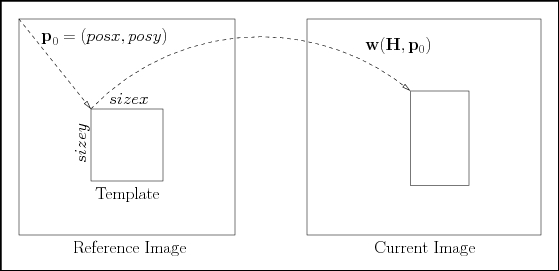
\includegraphics[width=1.0\textwidth]{tracking/figures/scale}
\caption{Translation and scaling of the reference template.}
\label{scale}
\end{center}
\end{figure}

In several applications, when tracking deformable objects it is better to fix the model to \lstinline$Rox_Tracking_Model_tu_tv_s$ or \lstinline$Rox_Tracking_Model_tu_tv_su_sv$.

% \subsubsection{Setting the parameters for tracking in the whole image or for target identification}
% \label{sss:tracking_params_ident}
% When the target make very large displacement in the image, it is sometimes necessary to search the target in the whole image. The same problem can arise when the target is lost, occluded or out of the image and the it comes back in the camera field of view. \rox{} allows the user to identify the target by choosing several identification methods using the following function:
% \begin{lstlisting}
% rox_tracking_params_set_ident(Rox_Tracking_Params P, Rox_Sint ident)
% \end{lstlisting}
% Setting ident to 0 will disable the research. The methods 1 and 2 are more robust but slower. The methods 2 and 4 are faster but the identification success rate is lower.

% The research time in the whole image may be a time consuming step. Thus it is possible to reduce the computation time by setting a parameters that tell to \rox{} to reduce the size of the image before the research. The use can use the following function:
% \begin{lstlisting}
% rox_tracking_params_set_ident_full_image(Rox_Tracking_Params P, Rox_Bool ident_full_image)
% \end{lstlisting}
